%\documentclass[8pt, handout]{beamer}
%\usepackage{pgfpages} 								%Для распечатки
%\pgfpagesuselayout{2 on 1}[a4paper,border shrink=10mm]

\documentclass[8pt]{beamer}

\usepackage[english,russian]{babel}
\usepackage[utf8]{inputenc}
\usepackage{mflogo}
\usepackage{amsmath,amsfonts,amssymb}
\usepackage{euscript}
\usepackage{graphicx}
\usepackage{xcolor}
\usepackage{transparent}

\newcommand{\grad}{\mathrm{grad\,}}


\beamertemplatenavigationsymbolsempty

\usetheme{EastLansing}
\setbeamercovered{transparent}


\title[Функции многих переменных]{Математический анализ\\ Тема 6: Функции многих переменных}
\author[Выборный Е. В.]{Выборный Евгений Викторович\\ email: evybornyi@hse.ru}
\date{Москва 2016} 


\makeatletter
\setbeamertemplate{footline}{
    \leavevmode%
    \hbox{%
    \begin{beamercolorbox}[wd=.25\paperwidth, ht=2.5ex, dp=1ex, center]{author in head/foot}%
        \usebeamerfont{author in head/foot}%
        \insertshortauthor
    \end{beamercolorbox}%
    \begin{beamercolorbox}[wd=.5\paperwidth,ht=2.5ex,dp=1ex,center]{title in head/foot}%
        \usebeamerfont{title in head/foot}\insertshorttitle
    \end{beamercolorbox}%
    \begin{beamercolorbox}[wd=.25\paperwidth,ht=2.5ex,dp=1ex,right]{date in head/foot}%
        \usebeamerfont{date in head/foot}\insertshortdate{}\hspace*{2em}
        \insertframenumber{} / \inserttotalframenumber\hspace*{2ex}
    \end{beamercolorbox}}%
    \vskip0pt%
}
\makeatother

\makeatletter
\setbeamertemplate{title page}
{
\centering
 \usebeamerfont{author}\insertauthor
 \vfill
 \begin{beamercolorbox}[rounded=true,shadow=true,sep=8pt,center]{title}
  \usebeamerfont{title}\inserttitle
 \end{beamercolorbox}
\vfill
\centering
\insertdate\par
 \vskip0.2em
}
\makeatother

\begin{document}
%\parindent=1.5em %красная строка

\begin{frame}
\titlepage
\end{frame}

\begin{frame}{Пространство $\mathbb{R}^n$}
\begin{block}{Определение. Вещественное $n$-мерное пространство $\mathbb{R}^n$}
Множество упорядоченных наборов из $n$ действительных чисел называют {\bf вещественным $n$-мерным пространством} $\mathbb{R}^n$:
$$x=(x_1,\ x_2,\ldots,\ x_n)\in \mathbb{R}^n.$$
Эти наборы чисел из $\mathbb{R}^n$ называют точками или векторами. В $\mathbb{R}^n$ определена сумма векторов и операция умножения вектора на число:
$$x+y = (x_1,\ x_2,\ldots,\ x_n)+(y_1,\ y_2,\ldots,\ y_n) = (x_1+y_1,\ x_2+y_2,\ldots,\ x_n+y_n),$$
$$\alpha x = \alpha\cdot (x_1,\ x_2,\ldots,\ x_n) = (\alpha x_1,\ \alpha x_2,\ldots,\ \alpha x_n).$$
Определено понятие расстояния между точкам:
$$d(x,y) = \|x-y\| = \sqrt{(x_1-y_1)^2+\cdots+(x_n-y_n)^2}.$$
Выполнено неравенство треугольника:
$$\|x+y\|\le \|x\|+\|y\|.$$
\end{block}
\end{frame}

\begin{frame}{Шар в $\mathbb{R}^n$}
Ключевым понятием для определения сходимости в одномерном случае была $\varepsilon$-окрестность точки $a$. Определим аналогичные понятия в многомерном пространстве $\mathbb{R}^n$.

\begin{block}{Определение. Шар в $\mathbb{R}^n$}
{\bf Открытым шаром} в $\mathbb{R}^n$ с центром в точке $a$ и радиусом $r$ называют множество точек $x\in \mathbb{R}^n$, удовлетворяющих условию
$$\|x-a\|< r\ \iff\ (x_1-a_1)^2+\cdots+(x_n-a_n)^2 < r^2.$$
Иногда это множество называют $r$-окрестностью точки $a$, сохраняя обозначение $O_r(a)$. Тогда {\bf проколотой $r$-окрестностью} точки $a$, называют множество точек:
$$\dot O_r(a) = O_r(a)\setminus \{a\} = 
\left\{ x\in\mathbb{R}^n\mid 0<\|x-a\|<r \right\}.
$$ 
\end{block}
\begin{block}{Определение. Ограниченное множество}
Множество $A\subset\mathbb{R}^n$ называется {\bf ограниченным}, если $A$ полностью лежит в некотором шаре. В этом случае существует $R$ такое, что
$$\|x\|<R\quad \forall x\in A.$$
\end{block}
\end{frame}

\begin{frame}{Предел последовательности точек}

\begin{block}{Определение. Предел последовательности точек}
Говорят, что последовательность точек $\{x^{(k)}\}$, $x^{(k)}\in\mathbb{R}^n$ сходится к точке $y\in\mathbb{R}^n$, пишут~$x^{(k)}\to y$, если к нулю стремится расстояние между $y$ и $x^{(k)}$ при $k\to+\infty$:
$$\lim_{k\to+\infty} d(y,\ x^{(k)}) = 0.$$
Эквивалентные записи имеют вид:
$$\forall\varepsilon>0\ \exists N:\quad x^{(k)}\in O_\varepsilon(y) \quad \forall k\ge N.$$ 
$$\forall\varepsilon>0\ \exists N:\quad \|x^{(k)} -y\|<\varepsilon \quad \forall k\ge N.$$
Таким образом, последовательность точек стремится к $y$ тогда и только тогда, когда в любом открытом шаре с центром в точке $y$ лежит бесконечно много точек последовательности, а вне его --- лишь конечное число.
\end{block}
\begin{block}{Упражнение}
Докажите, что множество точек сходящейся последовательности является ограниченным.
\end{block}
\end{frame}

\begin{frame}{Предел последовательности точек}

\begin{block}{Предложение}
Сходимость последовательности точек $\{x^{(k)}\}$ к точке $y$ эквивалентна сходимости координат точек $x^{(k)} = ( x_1^{(k)},\ldots,x_n^{(k)})$ к координатам точки $y = (y_1,\ldots,y_n)$:
$$\lim_{k\to+\infty} x^{(k)} = y\quad \iff \quad 
\lim_{k\to+\infty}x_1^{(k)} = y_1,\ldots,\lim_{k\to+\infty}x_n^{(k)} = y_n.$$
\end{block}

\begin{block}{Доказательство}
Доказательство теоремы непосредственно следует из очевидных неравенств:
$$|x_j^{(k)} - y_j|\le \sqrt{(x^{(k)}_1-y_1)^2+\cdots+(x^{(k)}_n-y_n)^2} \le n\max_{1\le j\le n} |x_j^{(k)} - y_j|.$$
\end{block}

\begin{block}{Замечание}
Иногда в $\mathbb{R}^n$ вводят другое понятие расстояния по формуле:
$$\tilde d(x,\ y) = \max_{1\le j\le n} | x_j - y_j |.$$
Следовательно, сходимость последовательности точек относительно расстояния $d$ и $\tilde d$ эквивалентна.
\end{block}
\end{frame}


\begin{frame}{Открытые множества}
\begin{block}{Определение. Внутренние точки множества}
Точка $a\in A\subset\mathbb{R}^n$, которая принадлежат множеству $A$ вместе с некоторым открытым шаром с центром в точке $a$, называется {\bf внутренней точкой} множества $A$.
\end{block}
\begin{block}{Определение. Открытое множество}
Множество точек $A\subset\mathbb{R}^n$ называется {\bf открытым}, если для каждой точки $a\in A$ этого множества существует открытый шар с центром в точке $a$, который полностью лежит в $A$:
$$A\ \text{--- открыто }\iff\ \forall a\in A\ \exists r>0:\ O_r(a)\subset A.$$
Пустое множество $\emptyset$ полагается открытым по определению.
\end{block}
Таким образом, открытое множество --- это множество, которое полностью состоит из внутренних точек.
\begin{block}{Пример}
Открытый шар является открытым множеством. Действительно, $\forall x\in A= O_R(a)$ положим $r = R - \|x-a\|>0$. Тогда
$$y\in O_r(x) \ \Rightarrow\  \|y -a\| =\| y-x+x-a\|\le \|y-x\|+\|x-a\|<r+\|x-a\| = R\ \Rightarrow\ y\in A.$$
\end{block}
\end{frame}

\begin{frame}{Свойства открытых множеств}
\begin{block}{Свойства открытых множеств}
\begin{enumerate}
\item Все пространство $\mathbb{R}^n$ является открытым.
\item Любое объединение открытых множеств является открытым.
\item Конечное пересечение открытых множеств является открытым.
\end{enumerate}
\end{block}
\begin{block}{Замечание}
Пересечение бесконечного числа открытых множеств может не быть открыто. Например,
$$A_k = (-1/k,+1/k)\subset \mathbb{R},\qquad k=1,2,\ldots$$
Множества $A_k$ открыты, но
$$\bigcap\limits_{k=1}^{+\infty}A_k = \{ x\in\mathbb{R}\mid x\in A_k\ \forall k\} = \{0\},$$
а множество, состоящее только из одной точки, не является открытым.
\end{block}
\end{frame}

\begin{frame}{Замкнутые множества}
\begin{block}{Определение. Предельные и изолированные точки множества}
Точка $a \in\mathbb{R}^n$ называется {\bf предельной точкой} множества $A$ или точкой сгущения, если в любой окрестности точки $a$ существуют точки из множества $A$, отличные от $a$:
$$\forall r>0\quad O_r(a)\cap A\ne \{a\}.$$
Точка $a\in A$ называется {\bf изолированной точкой} множества $A$, если существует окрестность точки $a$, в которой нет других точек из множества $A$.
\end{block}
Предельные точки могут как принадлежать, так и не принадлежать рассматриваемому множеству.

\begin{block}{Определение. Замкнутое множество}
Множество называется {\bf замкнутым}, если оно содержит все свои предельные точки. Пустое множество считают замкнутым по определению.
\end{block}
\begin{block}{Предложение. Замкнутость в терминах последовательностей}
Множество замкнуто тогда и только тогда, когда предел любой сходящейся последовательности точек этого множества также принадлежит этому множеству.
\end{block}
\end{frame}

\begin{frame}{Свойства замкнутых множеств}
\begin{block}{Свойства замкнутых множеств}
\begin{enumerate}
\item Множество является замкнутым тогда и только тогда, когда его дополнение является открытым:
$$A\text{ --- замкнуто }\iff\ (\mathbb{R}^n\setminus A)\text{ --- открыто.}$$
\item Все пространство $\mathbb{R}^n$ является замкнутым.
\item Конечное объединение замкнутых множеств является замкнутым.
\item Любое пересечение замкнутых множеств является замкнутым.
\end{enumerate}
\end{block}
\begin{block}{Определение. Компакт}
Замкнутое ограниченное множество в $\mathbb{R}^n$ называют {\bf компактом}.
\end{block}
Понятие компакта является естественным обобщением понятия отрезка в многомерном пространстве.
\begin{block}{Предложение. Компактность в терминах последовательностей}
Множество является компактом тогда и только тогда, когда из любой последовательности точек множества можно выбрать подпоследовательность, сходящуюся к точке из заданного множества.
\end{block}
\end{frame}

\begin{frame}{Граница множества}
\begin{block}{Определение. Граница множества}
Точка $x\in\mathbb{R}^n$ называется {\bf граничной точкой} для множества $M\subset \mathbb{R}^n$, если в любой окрестности точки $x$ есть как точки из множества $M$, так и точки не принадлежащие $M$. Граничные точки могут принадлежать или не принадлежать множеству $M$.
\vskip1em
Множество всех граничных точек для заданного множества $M$ называют {\bf границей} $M$ и обозначают $\partial M$.
\end{block}
Несложно доказать, что замкнутое множество всегда содержит свою границу. 
\vskip1em
Объединение множества и его границы всегда является замкнутым. Это множество называют замыканием множества $M$ и обозначают
$$\bar M = M\cup \partial\, M.$$
\vskip-1.3em
\begin{block}{Пример}
Несложно найти границы следующих множеств:
$$\partial\, [a,b] = \{a,\ b\},\qquad \partial\, (a,\ b) = \{a,\ b\};$$
$$\partial\, O_r(a) = \{ x\in\mathbb{R}^n\mid \|x-a\|=r\},$$
$$\partial\, \mathbb{R}^n = \emptyset.$$
\end{block}

\end{frame}

\begin{frame}{Область}
\begin{block}{Определение. Связное множество}
Множество $M\subset\mathbb{R}^n$ является {\bf связным} (линейно связным), если для любой пары точек $x$ и $y$ из $M$ существует непрерывный путь (кривая), которая соединяет точки $x$ и $y$, и при этом полностью лежит в $M$.
\end{block}

\begin{block}{Определение. Область}
{\bf Областью} в $M\subset\mathbb{R}^n$ называют открытое связное множество.
\end{block}
\begin{center}
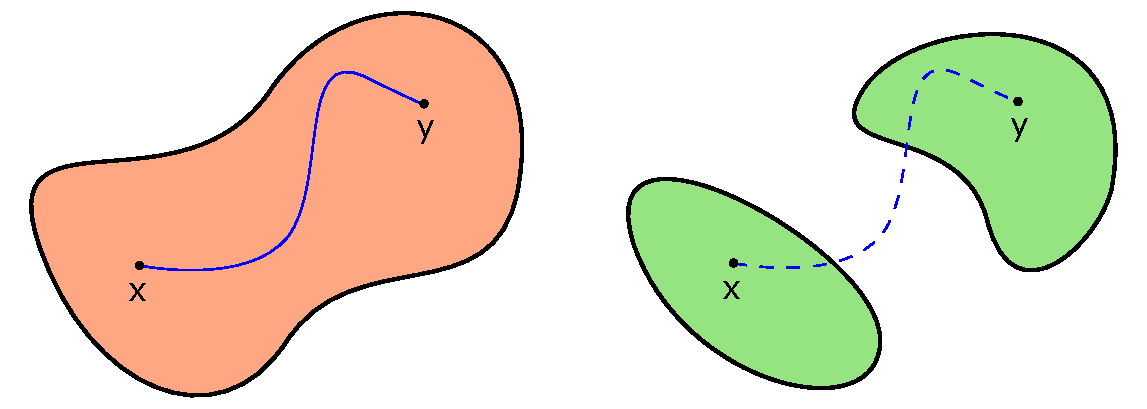
\includegraphics[scale=0.4]{conected-set.pdf}
\end{center}
Множество, изображенное на рисунке слева, является связным, а множество, изображенное справа, не является связным (состоит из двух частей).
\end{frame}

\begin{frame}{Функция нескольких переменных}
\begin{block}{Определение. Функция нескольких переменных}
{\bf Числовой функцией нескольких переменных} называют отображение $f:\ E\to \mathbb{R}$, где $E\subset\mathbb{R}^n$~--- некоторое множество, называемое {\bf множеством определения} функции. Значение функции $f$ в точке $x\in E$ записывают, как $f(x) = f(x_1,\ldots, x_n)$, при этом $x_j$ называют независимыми переменными, а $z=f(x)$ --- зависимой переменной, так как ее значение определяется выбором точки $x$.
\end{block}
\begin{center}
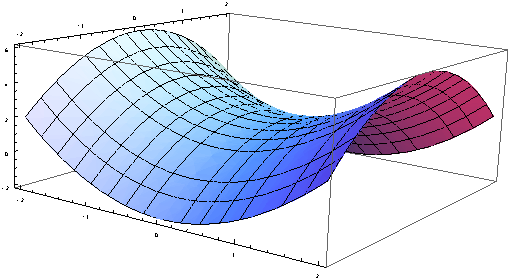
\includegraphics[scale=0.8]{Plot3D.pdf}
\end{center}
При рассмотрении функций двух переменных $z=f(x,y)$ можно рассматривать график функции как поверхность $\Gamma$ в трехмерном пространстве $\mathbb{R}^3$:
$$\Gamma = \{(x,y,z)\mid z=f(x,y),\ (x,y)\in E\}.$$
\end{frame}

\begin{frame}{Линии уровни}
Другой способ визуально представить функцию двух независимых переменных --- это рассмотреть семейство кривых на плоскости, вдоль которых функция является постоянной
$$f(x,y) = const$$
Данные кривые называют {\bf линиями уровня} для функции $f$.
\begin{center}
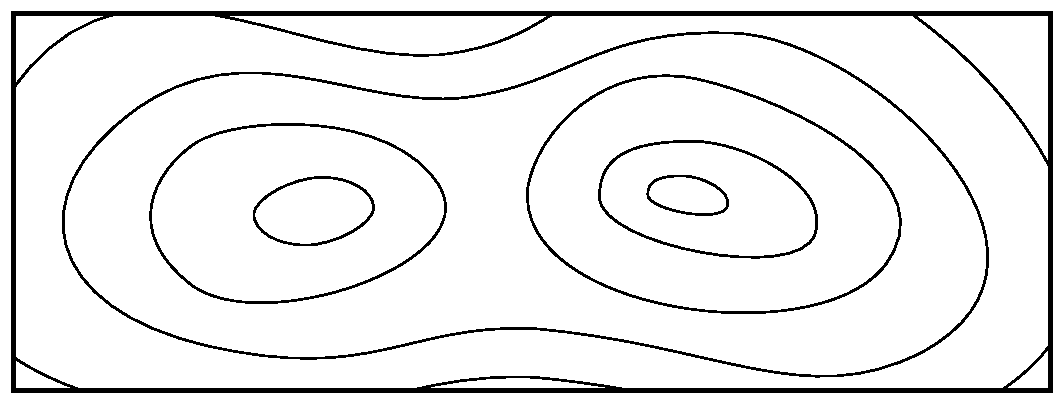
\includegraphics[scale=0.5]{cp.pdf}
\end{center}
\end{frame}

\begin{frame}{Предел функции}
\begin{block}{ Определение. Предел функции}
Пусть функция $f$ определена в некоторой проколотой окрестности точки $a\in\mathbb{R}^n$. Говорят, что число $f_0$ является {\bf пределом} $f(x)$ при $x\to a$, если
$$\forall \varepsilon>0\ \exists \delta>0:\quad |f(x) - f_0|<\varepsilon,\ \forall x\in \dot O_\delta(a).$$
В этом случае пишут $\displaystyle \lim_{x\to a}f(x) = f_0$. 

В случае двух переменных иногда пишут
$$\lim_{x\to x_0,\ y\to y_0} f(x,y) = f_0,$$
а соответствующий предел называют двойным.
\vskip0.5em
Как и в одномерном случае, можно определить сходимость в терминах последовательностей (по Гейне).
\vskip0.5em
Предел $f(x)$ равен $f_0$ при $x\to a$ тогда и только тогда, когда для любой сходящейся к $a$ последовательности точек $\{x^{(k)}\}$ из проколотой окрестности точки $a$ последовательность значений функции в этих точках $f(x^{(k)})$ сходится к $f_0$:
$$\forall \{x^{(k)}\}:\ x^{(k)}\to a,\ x^{(k)}\ne a\ \Rightarrow \ f(x^{(k)})\to f_0.$$
По аналогии с одномерным случаем определяются и бесконечные пределы функций.
\end{block}
\end{frame}

\begin{frame}{Предел функции}
Пусть функция $f$ определена на множестве $M$ и точка $a$ является предельной точкой множества  $M$. Тогда уместно говорить о стремлении $x\to a$ при условии $x\in M$, $x\ne a$.
\begin{block}{ Определение. Предел функции по множеству}
Говорят, что число $f_0$ является пределом функции $f(x)$ при $x\to a$ по множеству $M$ ($x\to a,\ x\in M$), если
$$\forall \varepsilon>0\ \exists \delta>0:\quad |f(x) - f_0|<\varepsilon,\ \forall x\in \dot O_\delta(a)\cap M.$$
В этом случае пишут $\displaystyle \lim_{x\to a,\ x\in M}f(x) = f_0$. 
\end{block}
Частным случаем предела по множеству служат односторонние пределы функции одной переменной.
\end{frame}

\begin{frame}{Непрерывность функции}
\begin{block}{Определение непрерывности в точке}
Говорят, что функция $f(x)$, определенная в некоторой окрестности точки $A\in\mathbb{R}^n$, {\bf непрерывна в точке} $x=A$, если
$$\exists\ \lim_{x\to A}f(x) = f(A).$$
\end{block}
\vskip-0.5em
\pause
Предположим, что функция определена на множестве $M$ и точка $A\in M$ является предельной точкой этого множества. Если точка $A$ не является внутренней для множества~$M$, а принадлежит его границе, то рассматривают следующие определение непрерывности:
\pause
\begin{block}{Определение непрерывности по множеству}
Говорят, что функция $f(x)$, определенная на множестве $M\subset\mathbb{R}^n$, {\bf непрерывна по множеству} $M$ в точке $x=A$, если
$$\exists\ \lim_{x\to A,\ x\in M}f(x) = f(A).$$
Функция считается по определению непрерывной в изолированных точках множества $M$.
\end{block}
\end{frame}

\begin{frame}{Непрерывность функции}
\begin{block}{Определение непрерывности по множеству}
Говорят, что функция $f(x)$, определенная на множестве $M\subset\mathbb{R}^n$, {\bf непрерывна} на множестве $M$, если она непрерывна в каждой точке множества  $M$.
\end{block}
\pause
Свойства непрерывных функций нескольких переменных во многом совпадают со свойствами непрерывных функций одной переменной.
\begin{block}{Свойства непрерывных функций}
\begin{enumerate}
\item Сумма и произведение непрерывных функций непрерывны. Частное непрерывных функций заведомо непрерывно, если делитель (знаменатель) не обращается в ноль.
\item Композиция непрерывных функций непрерывна.
\item Элементарные функции непрерывны на своем множестве определения.
\end{enumerate}
\end{block}
\pause
\begin{block}{Теорема Вейерштрасса}
Пусть функция $f(x)$ непрерывна на компакте $K\subset\mathbb{R}^n$. Тогда она ограничена на множестве~$K$ и достигает на нем своей верхней и нижней грани:
$$\exists x_{min}\in K:\quad f(x_{min}) = \inf_{x\in K}f(x),$$
$$\exists x_{max}\in K:\quad f(x_{max}) = \sup_{x\in K}f(x).$$
\end{block}
\end{frame}


\begin{frame}{Частные производные. Определение}
Рассмотрим функцию $f(x) = f(x_1,\ldots,x_n)$, заданную в окрестности точки $x^0=(x^0_1,\ldots,x^0_n)\in\mathbb{R}^n$. Тогда можно рассмотреть функцию одной переменной $x_k$, фиксировав остальные переменные:
$$\phi(x_k)=f(x^0_1,\ldots, x_{k-1}^0, x_k,x_{k+1}^0,\ldots,x^0_n).$$
Для определения скорости изменения значения функции $f(x)$ при изменении только одной переменной $x_k$ можно рассмотреть производную функции $\phi(x_k)$. Эту производную называют {\bf частной производной} функции $f$ по переменной $x_k$ в точке $x^0$ и обозначают:
$$ \frac{\partial f(x)}{\partial x_k}\Big|_{x=x^0} = \frac{\partial}{\partial x_k}\Big|_{x=x^0}f(x) = \frac{\partial f(x_0)}{\partial x_k}=\frac{\partial f}{\partial x_k}(x^0) = f'_{x_k}(x^0)=f_{x_k}(x^0) = \partial_k f(x_0).$$
\vskip-0.5em
\begin{block}{Определение}
Говорят, что функция $f$, определенная в окрестности точки $x^0\in\mathbb{R}^n$, имеет {\bf частную производную}  по переменной $x_k$ в точке $x^0$, если существует предел
$$\lim_{h\to 0}\frac{f(x^0_1,\ldots, x_{k-1}^0, x^0_k+h,x_{k+1}^0,\ldots,x^0_n) - f(x^0)}{h} = \frac{\partial f(x)}{\partial x_k}\Big|_{x=x^0}.$$
\end{block}
\end{frame}

\begin{frame}{Частные производные. Пример}
\begin{block}{Пример}
Вычислим частные производные функции трех переменных
$$u = x^2+2xy+\cos(x z).$$
Тогда
$$\begin{array}{l}
\frac{\partial u}{\partial x} = 2x+2y-\sin(xz)\, z;\\[0.8em]
\frac{\partial u}{\partial y} = 2x;\\[0.8em]
\frac{\partial u}{\partial z} = -x\sin(x z).
\end{array}$$
В данном случае вычисления производились в произвольной точке $(x,y,z)\in\mathbb{R}^3$. Тогда при дифференцировании по одной из переменных все остальные переменные можно считать постоянными.
\end{block}
\end{frame}

\begin{frame}{Дифференцируемость}
\begin{block}{Определение. Дифференцируемая функция}
Говорят, что функция $f$, определенная в окрестности точки $x^0\in\mathbb{R}^n$, {\bf дифференцируема} в точке $x^0$, если для любого достаточно маленького приращения $\Delta x$ переменной $x$:
$$\Delta x = \left( \Delta x_1,\ldots,\Delta x_n\right),$$
приращение значения функции представимо в виде:
$$\Delta f(x^0) = f(x^0+\Delta x) - f(x^0) = \sum_{k=1}^n A_k\, \Delta x_k + o\left(\|\Delta x\|\right),$$
где $A_k$ --- постоянные.
\vskip1em
Линейную часть приращения функции называют {\bf дифференциалом} и обозначают:
$$df\!\left(x^0\right)(\Delta x) = \sum_{k=1}^n A_k\, \Delta x_k.$$
Дифференциал является линейной формой порядка $n$, как функция от $\Delta x$, а также неявно зависит от выбора точки $x^0$.
\end{block}
\end{frame}

\begin{frame}{Дифференцируемость}
\begin{block}{Теорема. Необходимое условие дифференцируемости}
Пусть функция $f$ дифференцируема в точке $x^0\in\mathbb{R}^n$ и 
$$df\!\left(x^0\right)(\Delta x)  = \sum_{k=1}^n A_k\, \Delta x_k.$$
Тогда у функции $f$ существуют частные производные по всем переменным $x_k$ в точке $x^0$ и
$$A_k = \frac{\partial f}{\partial x_k}\!\left(x^0\right).$$
\end{block}
Таким образом, для дифференцируемости функции $f$ необходимо наличие у нее всех частных производных в заданной точке. 
\end{frame}

\begin{frame}{Дифференцируемость}
В одномерном случае существования производной было вполне достаточно для дифференцируемости функции, но в многомерном случае это уже не так.
\begin{block}{Упражнения}
\begin{itemize}
\item Проведите доказательство теоремы о необходимом условии дифференцируемости, аналогично доказательству в одномерном случае.
\item Докажите, что дифференцируемая функция непрерывна.
\item Покажите, что функция
$$f(x,y) = \frac{xy}{x^2+y^2},\quad f(0,0) = 0,$$
не является дифференцируемой, но имеет частные производные в точке $(0,0)$. Покажите, что эта функция не является даже непрерывной.
\end{itemize}
\end{block}
\end{frame}

\begin{frame}{Дифференцируемость}
Вычислим дифференциал функции 
$$u(x_1,\ldots,x_n) = x_k.$$
Тогда
$$u(x+\Delta x) - u(x) = \left(x_k+\Delta x_k\right) - x_k = \Delta x_k.$$
Следовательно, дифференциал имеет вид
$$du(x)(\Delta x) = dx_k(\Delta x) = \Delta x_k.$$
Таким образом, общую формулу для дифференциала функции $f$ можно переписать в виде:
$$df(x^0) = \sum_{k=1}^n \frac{\partial f}{\partial x_k}\!\left(x^0\right)\, dx_k.$$
\begin{block}{Упражнение}
Проверьте, что
$$d\left(\sqrt{x^2+y^2}\right) = \frac{xdx+ydy}{\sqrt{x^2+y^2}}.$$
\end{block}
\end{frame}

\begin{frame}{Дифференцируемость. Достаточное условие}
\begin{block}{Теорема. Достаточное условие дифференцируемости}
Пусть все частные производные $\displaystyle \frac{\partial f}{\partial x_k}$ функции $f(x)$ определены в окрестности точки $x_0$ и непрерывны в точке $x^0$. Тогда функция $f$ является дифференцируемой в точке $x_0$.
\end{block}
\vskip-0.5em
\begin{block}{Доказательство}
Проведем доказательство для $n=2$. Пусть $f = f(x,y)$. Тогда, применяя формулу конечных приращений, получаем:
\begin{multline*}
\Delta f = f(x,y) - f(x_0,y_0) = f(x,y) - f(x,y_0) + f(x,y_0) - f(x_0,y_0) =\\=
\frac{\partial f}{\partial y}(x,\eta)(y-y_0) +\frac{\partial f}{\partial x}(\xi,y_0)(x-x_0).
\end{multline*}
Из непрерывности частных производных следует, что
$$\frac{\partial f}{\partial y}(x,\eta) = \frac{\partial f}{\partial y}(x_0,y_0)+o(1),\qquad \frac{\partial f}{\partial x}(\xi,y_0) = \frac{\partial f}{\partial x}(x_0,y_0)+o(1).$$
Таким образом,
$$\Delta f = \frac{\partial f}{\partial x}(x_0,y_0)\Delta x+\frac{\partial f}{\partial y}(x_0,y_0)\Delta y + o\left(|x-x_0|\right)+o\left(|y-y_0|\right).$$
%Из неравенства
%$$|x-x_0|+|y-y_0|\le 2\sqrt{(x-x_0)^2+(y-y_0)^2}.$$
%следовательно
%$$o\left(|x-x_0|\right)+o\left(|y-y_0|\right) =o\left(|x-x_0|+|y-y_0|\right) = o\left(\sqrt{(x-x_0)^2+(y-y_0)^2}\right).$$
\end{block}
\end{frame}

\begin{frame}{Частные производные. Градиент}
\begin{block}{Определение. Градиент}
Если функция $f(x)$, $x\in\mathbb{R}^n$, имеет частные производные по всем переменным ($n$ штук) в фиксированной точке $x^0$, то числовой вектор
$$\grad f\, \Big|_{x=x^0} = \left(\frac{\partial f}{\partial x_1}\left(x^0\right),\ldots, \frac{\partial f}{\partial x_n}\left(x^0\right)\right)$$
называют {\bf градиентом} функции $f$ в точке $x^0$. То есть градиент --- это вектор, составленный из частных производных функции $f$ в точке $x^0$. 
\end{block}

\begin{block}{Определение. Производные высших порядков}
Если частная производная функции $f(x)$ по переменной $x_k$ определена в некоторой окрестности точки $x^0\in\mathbb{R}^n$, то можно определить {\bf частные производные второго порядка}:
$$\frac{\partial^2 f}{\partial x_k\partial x_m}\left( x^0 \right) = \frac{\partial}{\partial x_m}\Big|_{x = x^0} \frac{\partial f(x)}{\partial x_k},\quad k=1,\ldots, n,$$
как частные производные по переменной $x_m$ от функции $\displaystyle \frac{\partial f(x)}{\partial x_k}$. Аналогично определяются производные третьего порядка и далее.
\end{block}
\end{frame}

\begin{frame}{Частные производные. Пример}
\begin{block}{Пример}
Пусть
$$f = x^2+2xy.$$
Тогда
$$\begin{array}{ll}
\frac{\partial f}{\partial x} = 2x+2y;&
\frac{\partial f}{\partial y} = 2x;\\[0.8em]
\frac{\partial^2 f}{\partial x^2} = \frac{\partial}{\partial x}\left( 2x+2y\right)  =2;&
\frac{\partial^2 f}{\partial x \partial y} = \frac{\partial}{\partial y}\left( 2x+2y\right)  =2;\\[0.8em]
\frac{\partial^2 f}{\partial y \partial x} = \frac{\partial}{\partial x}\left( 2x \right)  =2;&
\frac{\partial^2 f}{\partial y^2} = \frac{\partial}{\partial y}\left(2x\right)  = 0.
\end{array}$$
Таким образом, для функции двух переменных существует четыре частных производных второго порядка. Они образуют матрицу $2\times2$. В общем случае размерности $n$ мы получим квадратную матрицу размера $n\times n$.
\end{block}
\end{frame}


\end{document}